\documentclass[preprint]{sigplanconf}

% The following \documentclass options may be useful:

% preprint      Remove this option only once the paper is in final form.
% 10pt          To set in 10-point type instead of 9-point.
% 11pt          To set in 11-point type instead of 9-point.
% numbers       To obtain numeric citation style instead of author/year.

\usepackage{amsmath}
\usepackage[pdftex]{graphicx}
\usepackage{tipa}
\usepackage{float}
\graphicspath{{images/}}

\newcommand{\cL}{{\cal L}}

\begin{document}

\special{papersize=8.5in,11in}
\setlength{\pdfpageheight}{\paperheight}
\setlength{\pdfpagewidth}{\paperwidth}

\conferenceinfo{CONF 'yy}{Month d--d, 20yy, City, ST, Country}
\copyrightyear{20yy}
\copyrightdata{978-1-nnnn-nnnn-n/yy/mm}
\copyrightdoi{nnnnnnn.nnnnnnn}

% Uncomment the publication rights you want to use.
%\publicationrights{transferred}
%\publicationrights{licensed}     % this is the default
%\publicationrights{author-pays}

\titlebanner{banner above paper title}        % These are ignored unless
\preprintfooter{short description of paper}   % 'preprint' option specified.

\title{High-Performance Persistent Graphs}
\subtitle{Storing graphs in key-mapped tries with lazy copying persistence}

\authorinfo{John Moody}
           {Colorado College '16}
           {john.moody@coloradocollege.edu}
\authorinfo{Benjamin Ylvisaker}
           {Assistant Professor, Colorado College}
           {ben.ylvisaker@coloradocollege.edu}

\maketitle

\begin{abstract}
In the world of persistent data structures, there exist few high performance graph libraries.
We propose in this paper a C library which stores an application-controlled persistent graph in a key-mapped trie, using chunking and lazy copying to conserve memory and increase performance.
We achieve -some stuff about time complexity that I haven't figured out yet and I have no results help-.
\end{abstract}

\category{CR-number}{subcategory}{third-level}

\keywords
persistent data structures, graphs, hash array mapped trie

\section{Introduction}
Graphs are one of the basic data structures in the programmer's arsenal.
A graph defines some number of nodes and edges, which connect nodes together.
Graphs have wide-ranging applications, from computational models to databases, networking and pathfinding.
To get information about nodes or edges in a graph within a program we typically use an array or some manner of key-value store.
A graph node's value is usually a list of adjacent nodes, which are either predecessors to that node or successors.
The value associated with an edge is typically just two identifiers for its predecessor and successor.
This paper explores storing graphs as a persistent data structure, which has some benefits over the traditional way of storing data for certain applications.
We will give a background on persistent data structures, and then propose a structure for persistent graphs with strong performance characteristics for various operations and optimized use of memory.
\section{Persistence}
What does it mean for data to be stored in a persistent way?
A piece of data is persistent if it does not change.
Consider a linked list in memory, Jeff:
\begin{figure}[H]
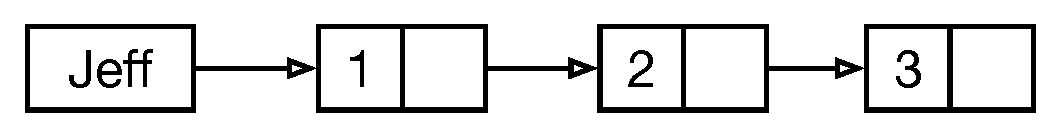
\includegraphics[scale=.35]{linkedlist}
\centering
\end{figure}
There are a number of ways to make an edit to this structure.
If we wanted to change the frontal value of Jeff from 1 to 5, and we do not need the original any longer, we may simply change it:
\begin{figure}[H]
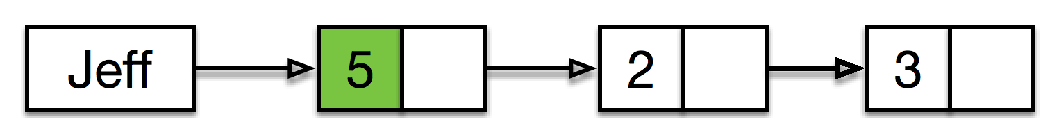
\includegraphics[scale=.35]{linkedlist2}
\centering
\end{figure}
If we want this notion of persistence to apply to Jeff, however, Jeff cannot change.
Instead, we need to come up with a way to change the front value of Jeff to 5 while keeping the original version of Jeff with 1 at the front intact.
Enter "Jeff'":
\begin{figure}[H]
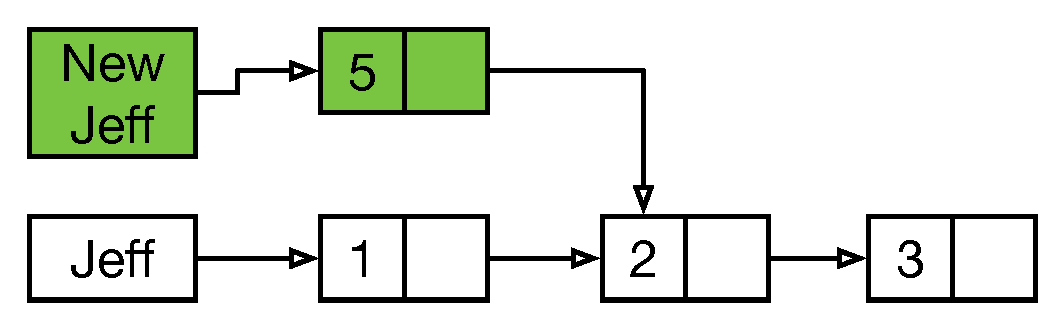
\includegraphics[scale=.35]{linkedlist3}
\centering
\end{figure}
Jeff, we notice, has not changed.
Jeff' preserves the parts of Jeff's structure that they have in common.
Persistent data structures, then, refer to structures like Jeff and Jeff', which, after being created, will always remain the same.

\subsection{Trees and Reference Counting}
Let us now consider an example using a simple binary search tree, where we have D, and a separate copy D':
\begin{figure}[H]
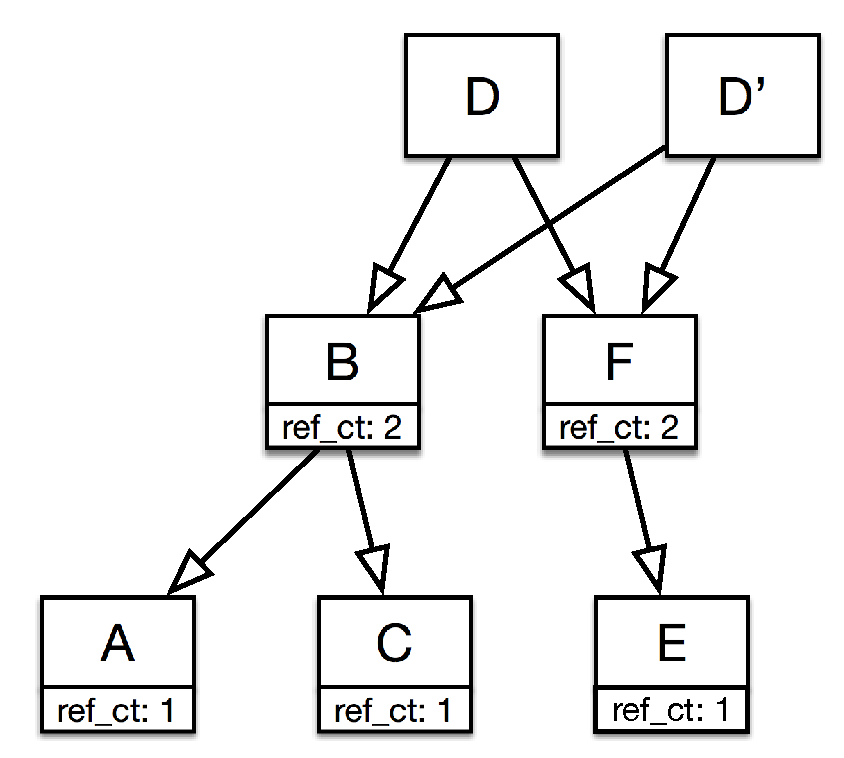
\includegraphics[scale=.43]{treefig}
\centering
\end{figure}
For us to be able to make edits to D' without changing D, we must introduce the concept of reference counting.
A reference count keeps track of how many objects point to a given node.
Here, since B and F have reference counts greater than one, we know that we can't modify those nodes without changing another version of the data structure.
Therefore, when we insert G into D', we will copy any nodes that have reference counts greater than one and adjust the tree as necessary:
\begin{figure}[H]
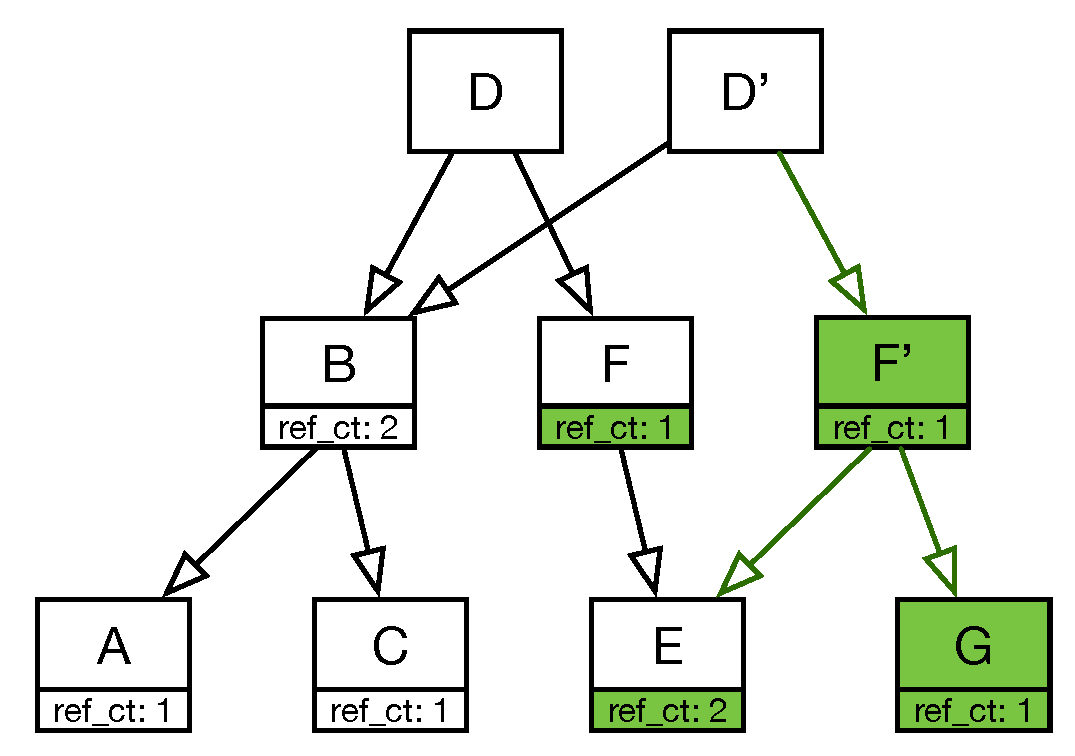
\includegraphics[scale=.43]{treefig2}
\centering
\end{figure}
The same concept applies in deleting or modifying nodes.
\subsection{Why?}
Why are persistent data structures interesting, or valuable?
In a broad sense, persistent data structures offer a way to do quick, cheap analysis on multiple versions of a large data structure.
In a mutable system, analyzing multiple versions of a data structure typically involves expensive wholesale copying of the structure, with no easy way to reverse changes that have been performed.
With persistent data structures, copies of a structure can be very small in size relative to the entire structure.
Reverting changes to that structure is simple, shown with the reference counting scheme from above.
If systems that perform analysis on large data sets are concerned with change to that data set over time, persistent data structures can be a powerful tool both in terms of how much space is used as well as performance.
Further, persistent data structures are more easily guaranteed to be thread-safe, since operations on persistent structures will never write to the parts of their structure that they share with other versions.
This characteristic makes persistent data structures easily operated on by multiple processes and threads, which dovetails with the increasing numbers of multi-core consumer processors.
Am I just talking out my ass here or should I say more stuff?
\section{Tries}
So, what is the best way to represent a graph persistently?
We know that whatever structure we use, if we want to efficiently store memory between versions, we imagine it to have elements of tree-like structure, with pointers between discrete parts.
A simple binary search tree is possible, and is used for some persistent graph libraries.
However, the use of a binary search tree introduces significant memory inefficiency.
If a node can only point to two other nodes, trees become very deep very quickly, which means lookups become costly.
Rather, our paper discusses the use of a wide-fanout key-mapped trie \textipa{[t\textturnr a\textsci]}, a derivative of the hash array mapped trie.
Our structure has the following characteristics:
\begin{itemize}
\item The library performs no hashing of values (nodes or edges of the graph).
Rather, each value is given a unique key either during or prior to insertion according to the current balance of the trie.
\item Values are stored only in leaves.
\item Wide fanout, to minimize trie depth.
\item Array compression, with bitmaps to indicate non-null positions.
\item Values are chunked together with their parent nodes.
\item Nodes without children are combined with their parents, to reduce the number of pointers.
\end{itemize}
The combining together of nodes without children with their parents means that nodes are effectively stored by the first unique bits of their key rather than the entire key itself.
To understand how this works, consider a hypothetical insert with keys of length 8, and 4-bit fanout among nodes, of a value with the key \texttt{11000110}.
Since our fanout is 4 bits, we will consider two bits of the key at a time in determining which branch of the trie to pursue.
\begin{figure}[H]
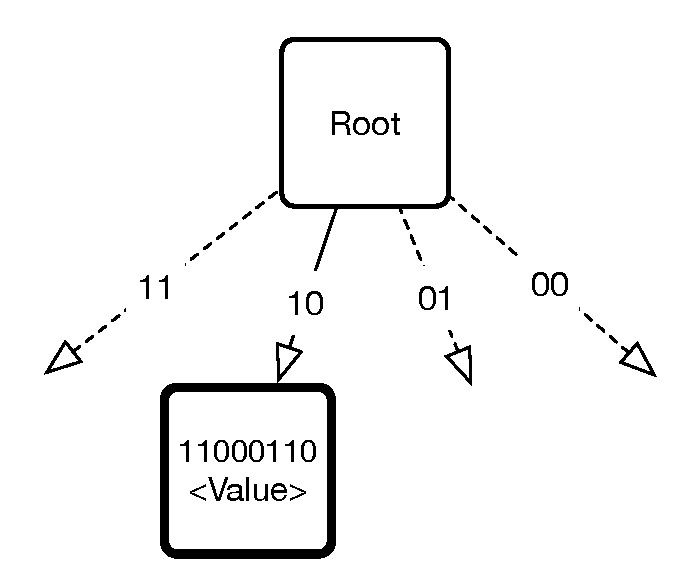
\includegraphics[scale=.5]{trie1}
\centering
\end{figure}
Here, we could create nodes that span the entire depth of the tree to insert the value, but since we would chunk these nodes together later, we will simply store the node in the root.
Since there are no other keys that begin with \texttt{10} in the set of keys, we don't need to create an interstitial node.
Inserting a node with a key that does begin with \texttt{10} results in the following adjustments:
\begin{figure}[H]
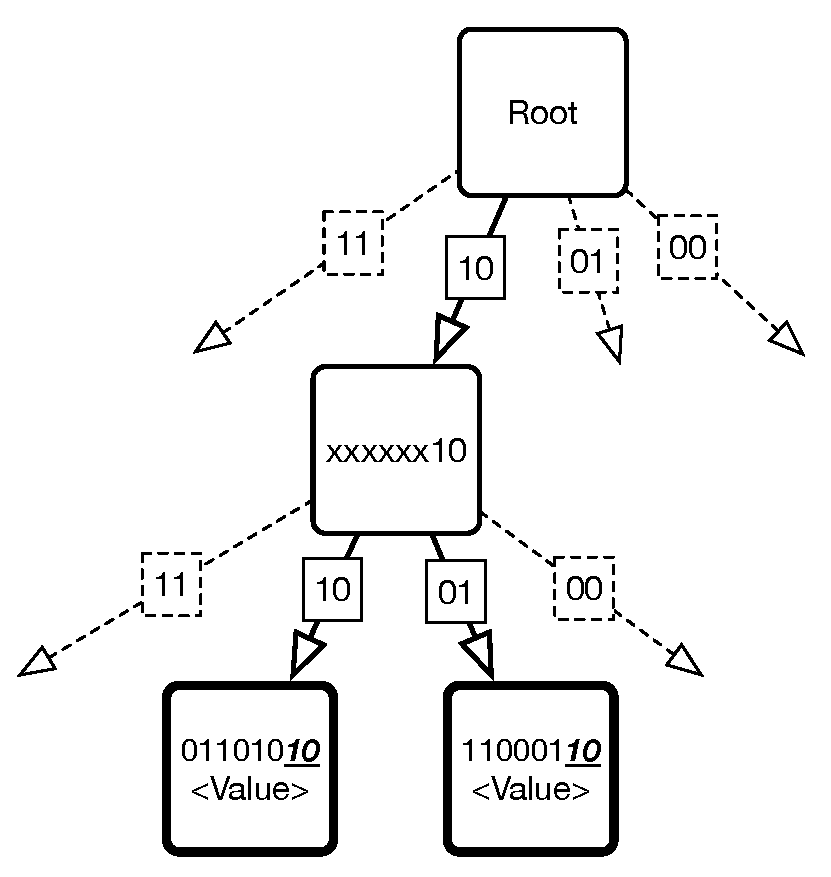
\includegraphics[scale=.5]{trie2}
\centering
\end{figure}
When we look up one of our nodes by the key, the library will examine the first two bits of the key, \texttt{10}.
Further, since all values are stored in the leaves of the trie, we will actually store the bolded values in arrays at the tail end of each parent node. Hence, our current trie will actually appear like this in memory:
\begin{figure}[H]
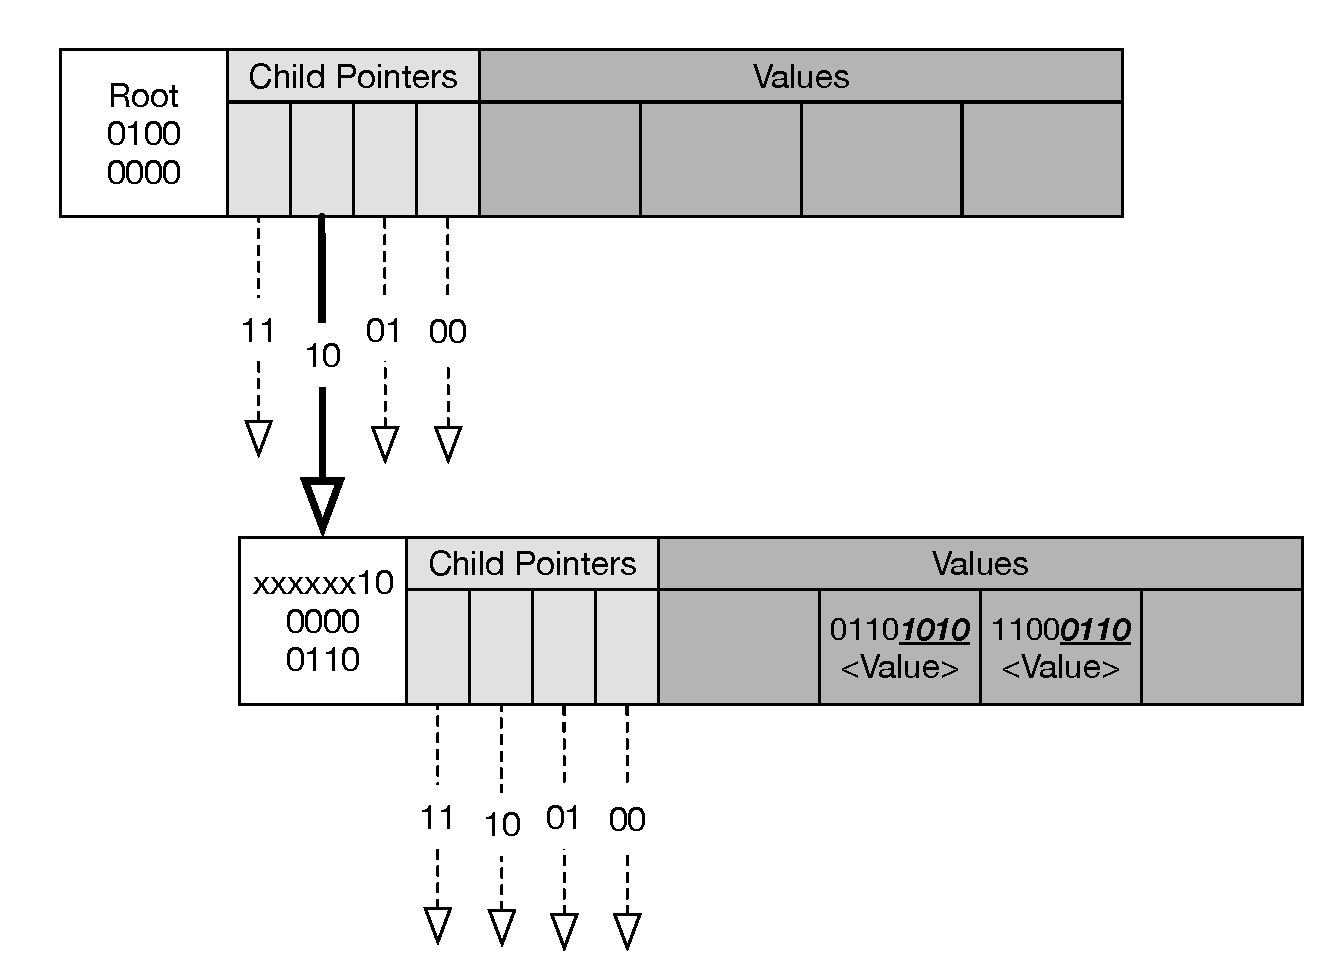
\includegraphics[scale=.47]{trie2actual}
\centering
\end{figure}
\subsection{Array Compression}
Storing these pointers and values in arrays means that, for nodes with low populations, we waste a lot of space on empty array slots.
We compensate for this with an array compression scheme borrowed from Phil Bagwell's hash array mapped trie.
In this scheme, the actual arrays that store pointers and values are dense and dynamically sized.
Each node stores two bitmaps that store data about which spots in our hypothetically complete array are occupied. 
If we want to access a value or pointer at a particular position, we will perform some bitwise arithmetic to determine in which dense array slot our desired value lies.
To illustrate an example, let us consider a bitmap 12 bits in length, which tells us about an array with seven values, \texttt{011011101010}.
For ease of comprehension, the array will be reversed so that the least significant bits of the bitmap correspond to the lowest indices in the array:
\begin{figure}[H]
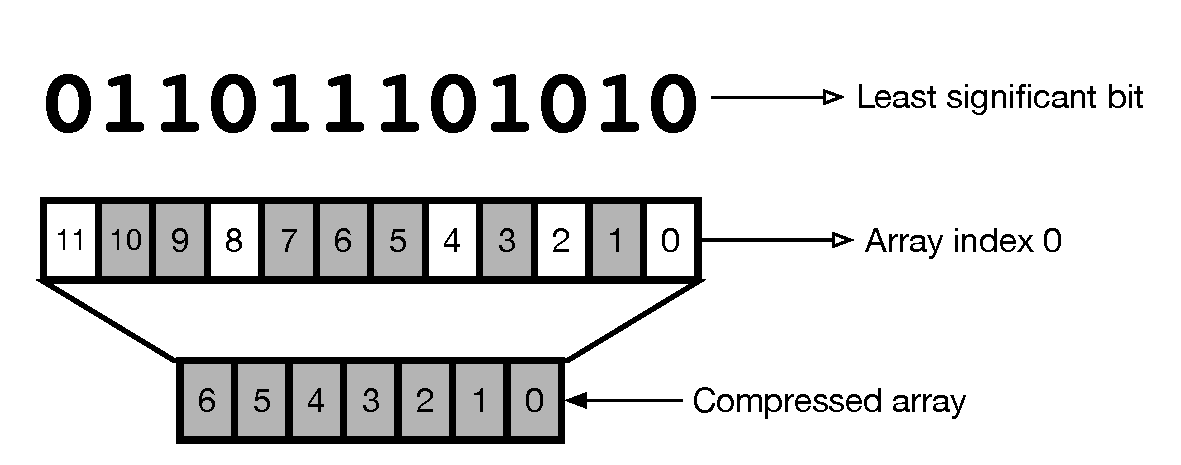
\includegraphics[scale=.43]{bitmask}
\centering
\end{figure}
The bitmap indicates that the keys 2, 4, 6, 7, 8, 10, and 11 are currently occupied by values.
Let's imagine the key we want to use for insertion or lookup is 9, or, in other words, that the five bits of the key we are concerned with are \texttt{01001}.
This means we want to check the 8th index of the hypothetical array.
To verify whether this spot is empty, we will simply bitwise \texttt{AND} together the bitmask and a number whose 8 least significant bits are 1s.
The number of 1s in the result represents how many spots are occupied in the compressed array prior to the one we want to insert into (or, in other words, the array index of our desired spot).
We will now use the population count instruction, which is built in to most modern processor architectures, to derive the index we need in our dense array, 5:
\begin{figure}[H]
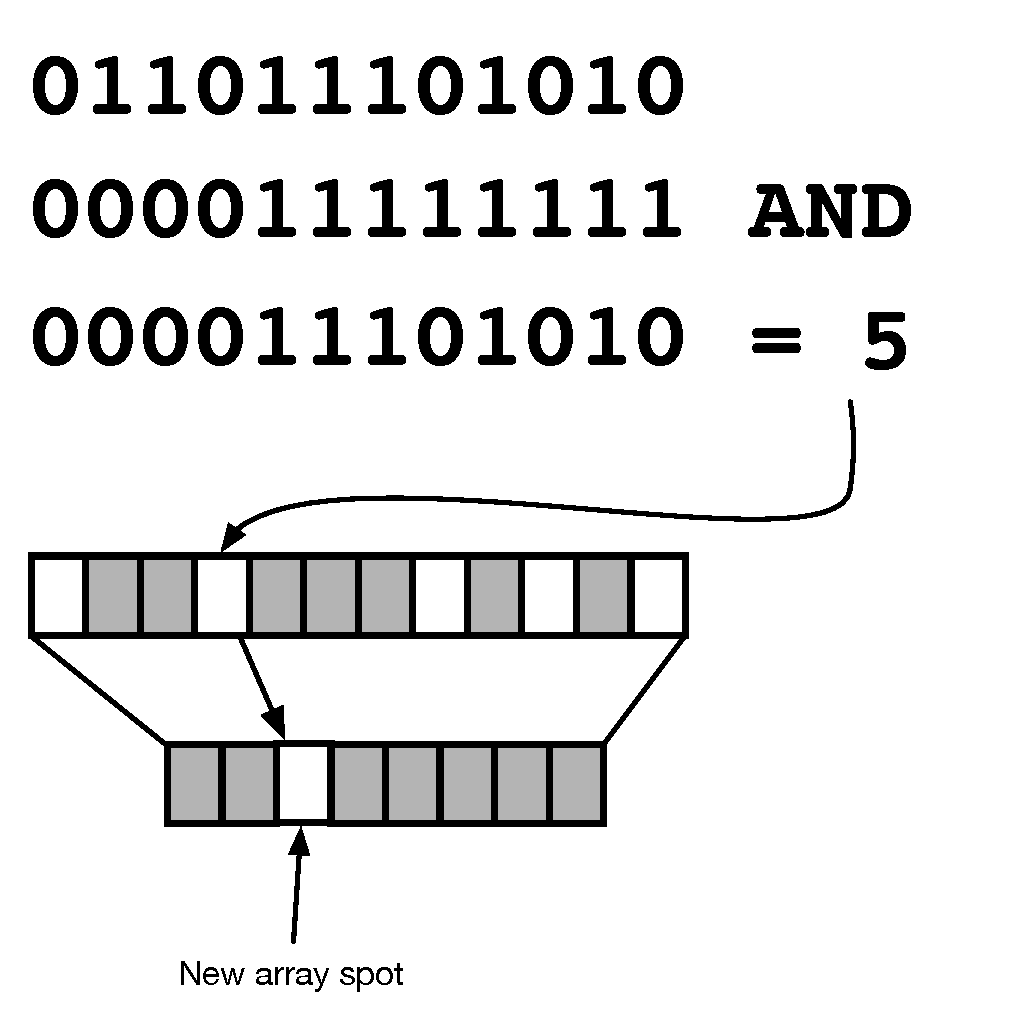
\includegraphics[scale=.45]{bitmask2}
\centering
\end{figure}
Using this scheme we conserve the memory that would normally be occupied by empty array slots.
This conservation is particularly important when we update the structure persistently, since creating copies of empty array slots would introduce large amounts of waste.
Let's take a look at our nodes in memory using the value bitmap from above, and the child bitmap \texttt{100010011001}.
Note that we have put the arrays back in the usual order to reflect how the values and pointers are actually stored in memory:
\begin{figure}[H]
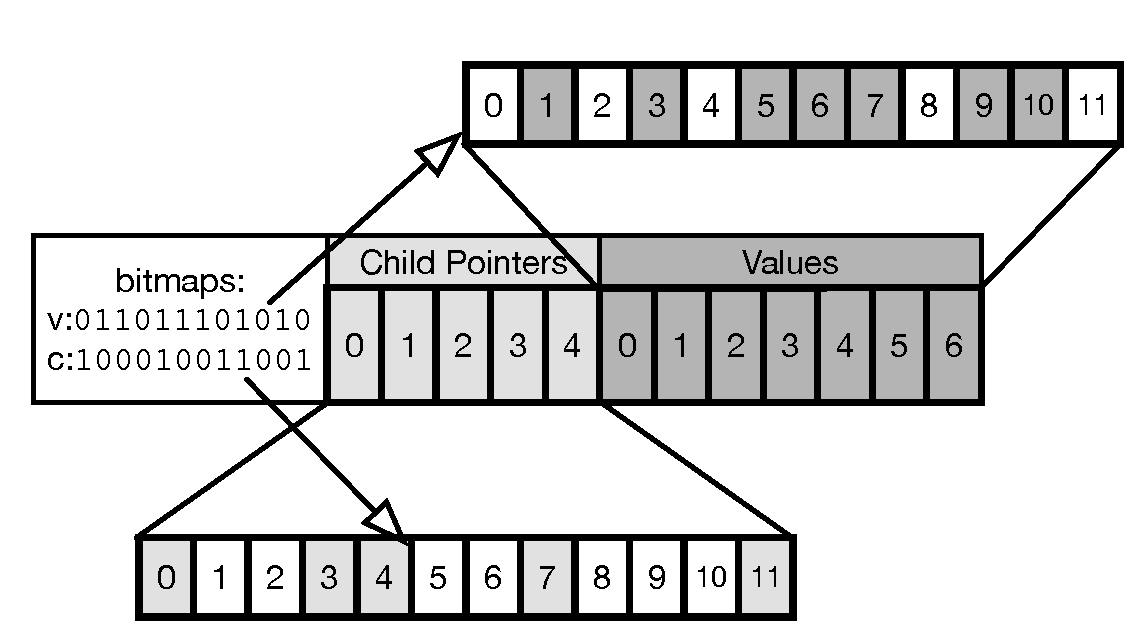
\includegraphics[scale=.45]{nodewithbitmaps}
\centering
\end{figure}
\subsection{Trie Balancing}
To ensure good asymptotics when looking up values at random in our graph, as might happen during a traversal of the graph, we want to keep our trie as balanced as possible.
'Balance,' in the context of tree-like structures, means that values are equally distributed in branches.
If no part of the trie is deeper than any other part, we have a uniform lookup speed for all values, ensuring that we don't spend a long time finding certain values nested deep in the trie.
For our trie to retain balance, we have to create keys for new values that place them in the appropriately least-populated section of the trie.
We employ a simple scheme which could be optimized for greater performance.
In this scheme, a node stores the index of the least populated of its children, as well as the total size of everything beneath that node in the trie.
After each discrete insertion or deletion from our trie, the total size value is adjusted for each node affected, and, if necessary, the index of the least populated node changed.
In this figure, a value of size 5 is inserted into the right-most branch of the trie, which causes a new least-populated child to be designated:
\begin{figure}[H]
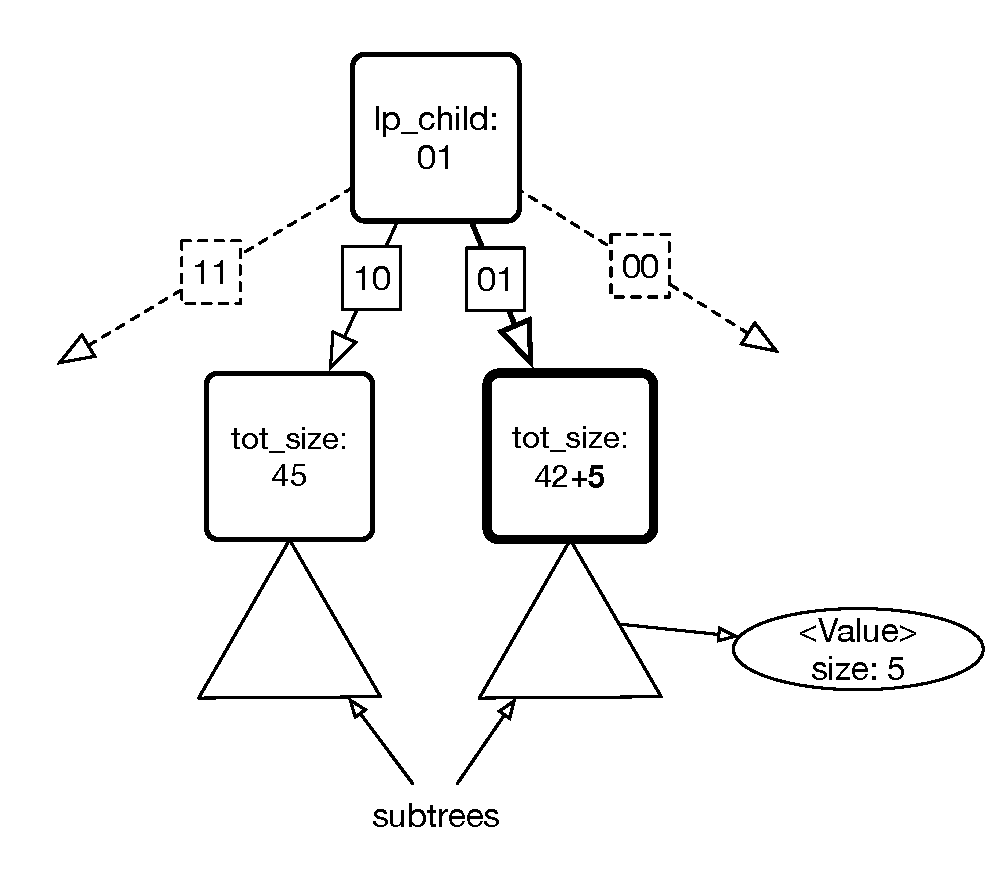
\includegraphics[scale=.45]{balancing}
\centering
\end{figure}
After the insert is performed, the child at 10 becomes the new least populated child:
\begin{figure}[H]
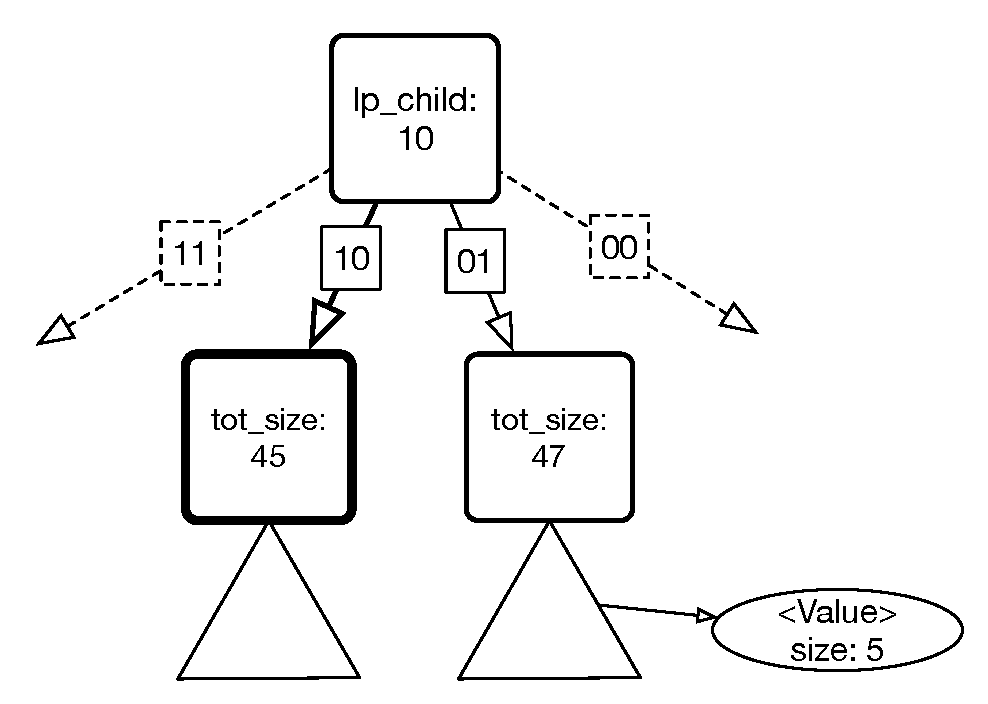
\includegraphics[scale=.45]{balancing2}
\centering
\end{figure}
This does some stuff to write performance that I'll talk about when I finish coding and testing it.
\subsection{Buffers}
With the densely packed arrays from section 3.1, every time we wish to insert into our trie structure, we need to resize the array of the node we insert into.
Since structs in C are not dynamically sized, the addition of a new value necessitates re-allocating the entire struct instance to compensate for the newly resized array.
This results in huge amounts of churning memory, which means very expensive writes.
To reduce the complexity and churn of the average write, we introduce \texttt{n}-sized buffers at the end of our dense arrays.
These buffers, which may be resized by the application, represent free space in which a node may store \texttt{n} values or children before the struct instance will be full and in need of reallocation.
This significantly decreases the amount of memory being allocated and freed on each insert on average. The exact effects of the various sizes of these buffers are detailed in our Results section.
Revisiting our diagram from the previous section, we can see how the buffers behave in our implementation:
\begin{figure}[H]
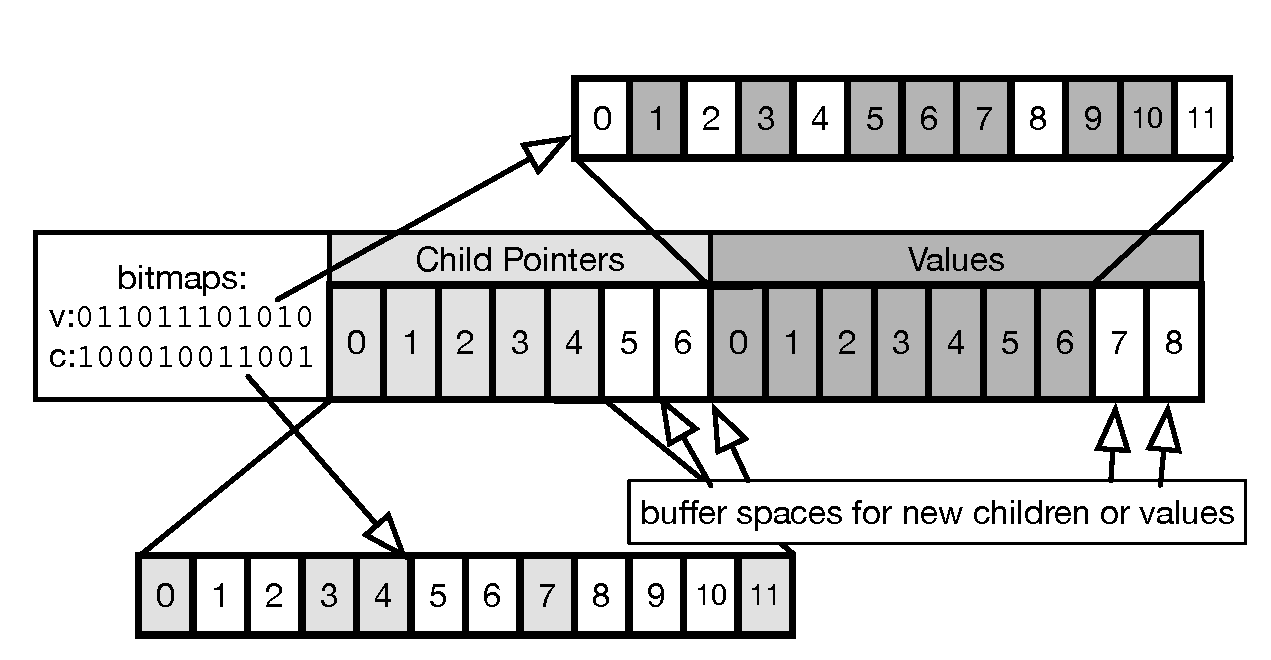
\includegraphics[scale=.42]{buffers}
\centering
\end{figure}
\subsection{Lazy Copying}
Next we will discuss the exact flavor of persistence that our library implements, ``lazy copying.''
Using lazy copying, an update to a trie structure \texttt{n} will, by default, be performed in place, without preserving the previous version. 
Creating a copy of \texttt{n} causes a copy of \texttt{n}, \texttt{n'}, to be created, and increments the reference counts of its children.
Thenceforth, if an update to to either \texttt{n} or \texttt{n'} changes a node with a reference count greater than one, that node is first copied to prevent other versions of the structure from being modified.
A high-level example of how this works is seen in the earlier Trees and Reference Counting section. \par
Our chunking together of values with nodes leads to redundancy using lazy copying.
If an update to a branch of the trie requires that branch to be copied, and the nodes in that branch are full of values, we will make many redundant copies of the values in that branch.
We consider this an acceptable tradeoff considering the advantages in read-performance associated with chunking and reducing our overall number of pointers, though this solution does increase our memory footprint as we modify persistent copies of our graph.
\section{Results}
We include tests that show our memory usage and read/write performance for mutable and persistent updates using various configurations of the library (32-bit fanout, 64-bit fanout, 16-bit fanout?).
Next, we include a comparison of random insertion/deletion performance and memory footprint for different values of \texttt{VALUE\_BUFFER\_SIZE} and \texttt{CHILD\_BUFFER\_SIZE}.
Lastly, for the time complexities of a random traversal of a randomly generated Erdos-Renyi graph, as well as a random sequence of insertions, deletions, and lookups, we compare to the Boost Graph Library included in C++.

\appendix
\section{Appendix Title}

This is the text of the appendix, if you need one.

\acks

Acknowledgments, if needed.

% We recommend abbrvnat bibliography style.

\bibliographystyle{abbrvnat}

% The bibliography should be embedded for final submission.

\begin{thebibliography}{}
\softraggedright

\bibitem[Smith et~al.(2009)Smith, Jones]{smith02}
P. Q. Smith, and X. Y. Jones. ...reference text...

\end{thebibliography}


\end{document}
